\subsection{Abstract Syntax}
\begin{figure}
	\center
	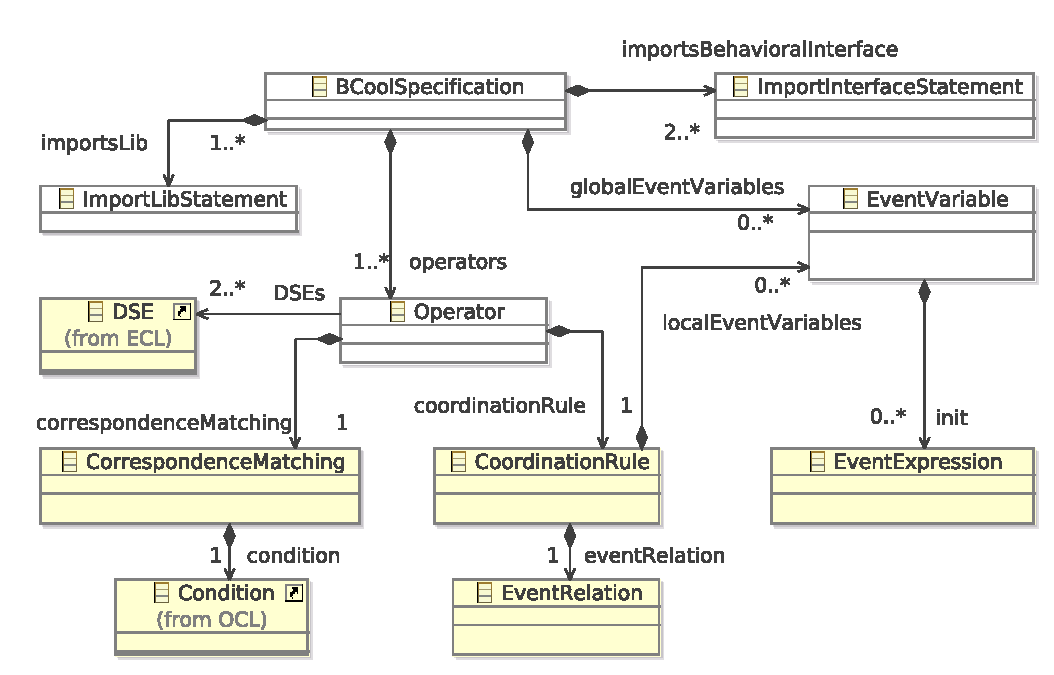
\includegraphics[width=.8\textwidth]{bcool/figs/BcoolMM}
	\caption{Simplified view of \bcool abstract syntax}
	\label{fig:bcool}
\end{figure}

\begin{itemize}
	\item The \bcool language is an implementation of the framework for coordination pattern approaches that we presented in Chapter~\ref{ch:framework}. A \bcool specification relies on operators to capture coordination patterns between languages. Operators are used to specify What, When and How instances of \dse (\mse) from different languages behavioral interfaces must be coordinated. To do so, each operator contains a correspondence matching and a coordination rule. These elements represent respectively the correspondence rule and the coordination rule presented in Chapter~\ref{ch:framework}. In this subsection, we present the syntactic elements of \bcool. To illustrate them, we define the operator for the running example between the language Activity and TFSM languages.
	
	\item The abstract syntax of the \bcool is defined by its metamodel (see Figure~\ref{fig:bcool}). The root element is a \emph{BCoolSpecification} that contains \emph{Operators}. Each operator refers to \dse to specify the event types it coordinates. In our implementation, we force operators to be defined between at least two event types. The \dse are extracted from the language behavioral interface that must be imported. A \bcool specification imports at least two  two language behavioral interface (\emph{importsInterfaceStatements}). The imported interface may belong to the same language.    
	
\end{itemize}


%The main element of \bcool (see Figure~\ref{fig:bcool}) is a \emph{BCoolSpecification} that contains language behavioral interfaces (\emph{importsInterfaceStatements}) and \emph{Operators}. The specification must import at least two language behavioral interfaces. Interfaces provide the \emph{DSE} needed for the coordination. The imported \dse serve as parameters for the operators. Then, an operator specifies what instances of these \dse are selected and how they are coordinated (the \emph{DSEs} reference). For instance, to build the running example, we synchronize FSMEvents and the starting of Actions. This is done by coordinating the instances of \dse \emph{occurs} and \emph{startAction} (see Appendix~\ref{ap:languages}). To do so, in a \bcool specification named \emph{SyncFSMEventsAndActions} (Listing~\ref{lst:bcoolrunningexample}: line 1), we import the language behavioral interface of TFSM and Activity (Listing~\ref{lst:bcoolrunningexample}: line 3 and 4). Then, we define the operator named \emph{SyncProduct} with \emph{occurs} and \emph{startAction} as parameters  (Listing~\ref{lst:bcoolrunningexample}: line 6). 

Each operator contains both a \emph{correspondenceMatching} and a \emph{coordinationRule}. The former relies on a Boolean \emph{Condition} defined as an OCL expression. It acts as a precondition for the coordination rule, \ie it is a predicate that defines when the coordination rule must be applied to the given parameters. To specify the predicate, it is possible to navigate through the context of the \dse and query a specific element used within the Boolean expression. For instance, for the running example, the condition selects pairs of instance of \dse \emph{occurs} and \emph{startAction} by looking at its attribute \emph{name} (Listing~\ref{lst:bcoolrunningexample}: line 7). %This corresponds with a correspondence that relies on a naming convention. We call such a correspondence implicit, however the correspondence may be explicit, we study that case in Section~\ref{subsubsec:explicitcorrespondence}.

The \emph{coordinationRule} specifies how the selected instances of \dse must be coordinated. To do so, the user must define \emph{EventRelation} and some \emph{EventVariables} (\emph{localEventVariables}).

\begin{lstlisting}[language=bcool,
caption={Synchronized product operator between the TFSM and Activity languages},
label={lst:bcoolrunningexample}, 
basicstyle=\scriptsize\ttfamily, backgroundcolor=\color{LGrey}, numbers=left, xleftmargin=2pt]
BCOoLSpec TFSM-fUMLOperators
ImportLib "facilities.moccml"
ImportInterface "activitySemantics.ecl" as activity
ImportInterface "TFSM.ecl" as tfsm

Operator SyncProduct(dse1 : activity::startAction, dse2 : tfsm::occurs)
CorrespondenceMatching: when(dse1.name = dse2.name)
CoordinationRule: RendezVous(dse1, dse2)
end operator
\end{lstlisting}

Event relations restrict the occurrences of the events on which it is applied. The actual parameters of the event relation can be some instances of \dse and/or some \emph{EventVariables}. For instance, in the running example we want a strong synchronization between FSMEvents and Actions. Thus, the coordination rule uses a ``rendez-vous'' relation between the selected instances of \dse \emph{occurs} and \emph{startAction} (see Appendix~\ref{ap:expressionandrelations}). As a result, all the occurrences of these events are forced to happen simultaneously. Figure~\ref{fig:runningrdv} shows the resulting coordination in the case of the coffee machine. The instance of \dse \emph{occurs} and \emph{startAction} happens simultaneously.

\begin{figure}[h]
	\center
	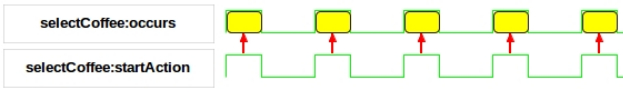
\includegraphics[width=.6\textwidth]{bcool/figs/runningrdv}
	\caption{Resulting coordination of the Coffee Machine by using the event relation Rendezvous}
	\label{fig:runningrdv}
\end{figure}
	

Lots of other relations, more or less complex can be defined, \eg \emph{Causality}, \emph{FIFO} or ad-hoc relations for specific protocols. For instance, Figure~\ref{fig:runningrunningcausality} illustrates the resulting coordination if we use the event relation \emph{Causality}. The definition of event relations is made in dedicated libraries, which must be imported (see Section~\ref{subsec:bcoollib}).

\begin{figure}[h]
	\center
	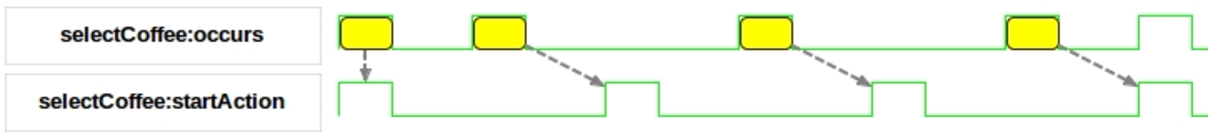
\includegraphics[width=.65\textwidth]{bcool/figs/runningcausality}
	\caption{Resulting coordination of the Coffee Machine by using the event relation Causality}
	\label{fig:runningrunningcausality}
\end{figure}